\chapter{Basic Concepts and Terminology}
\label{concepts}
In order to give a clear impression of the used terms and concepts by introducing and defining them in this chapter.

\textbf{Information Visualization}\\*
Information Visualization is the graphical representation of non-spatial or abstract data\cite{Keim}. In contrast to scientific visualization the data which is visualized in information visualization does not have an inherent 2D or 3D structure\cite{Shneiderman2008} and thus, no spatial relation. Usually abstract data comes in data tables with rows and columns. In Information Visualization columns are mapped to graphical attributes such as position, color, size, orientation, texture or hue. 
As business data usually is abstract, discrete and multi-variate\cite{Tegarden1999} the type of visualization for business data is Information Visualization.

\textbf{Visualization technique}\\*
The way how data variables are mapped to graphical primitives is called visualization technique. To avoid the redundant use of the term visualization we will call visualization techniques simply \textit{techniques} in the following work. Typical examples for techniques are bar charts, line charts or scatterplots. Thereby, every technique has its own characteristic in presenting data. These characteristics include the used visualization attributes, the mapping, the use of aggregation methods, dimensionality. Visualization characteristics are called the \textit{visual metaphor} of a technique\cite{Tegarden1999}. Each metaphor has its own strengths and weaknesses and its particular application. In this work we will focus on \textit{time-oriented data} and thus, only consider techniques for this cause. Moreover, we will only study stand-alone techniques: Techniques such as scatterplots which map data to a a graphical representation. In contrast to stand-alone techniques exist tools and systems. These involve several linked views and a often a specific UI in their design.
\\*

\textbf{Visual Data Exploration}\\*

\textbf{Time-oriented Data}\\*
Data which is linked to time\cite{Aigner2011} is called \textit{time-oriented data}. 




\textbf{Visualization Tools}\\*
While BI is defined as...\todo{Definition BI} data mining describes the extraction of patterns and models of the underlying data structure\cite{FerreiradeOliveira2003}. When data mining is used together with visualization data mining is based on automated algorithms which detect relevant patterns and display the results afterwards. In contrast, visual data exploration is a completely human guided process\cite{FerreiradeOliveira2003}. First data is displayed on the screen as a visualization and with the help of human visual capabilities new hypothesis are formed. Data visualization is a more general term for generating a graphical representation out of data and is used as well in BI, Analytics, data discovery as in visual analytics. 
Visualization tools display hundreds of items on the screen and offer interaction techniques such as zooming and filtering\cite{Shneiderman2008}.

\section{Business Information Visualization}\label{BIV}
Information Visualization 
Tools for Business Intelligence (BI) and Analytics, visualization, data discovery as well as for data mining continually gain importance in companies to assist humans to gain insights into their data. Although the differentiation between those tools is not selective and the terms are not clearly distinguished we can make the following differentiation: Data Mining tools allow automatic decision-making by applying algorithms to the data and extract patterns in an automatic way\cite{Goebel1999} while exploratory data analysis (EDA) tools are used to mine data with support of human input. We will use the definition of EDA tools if we speak of visualization tools in this work. As a pwc-survey showed eventhough automatic ways for decision support exists data analysis stil relies on human judgement and thus\cite{PwC2016}, visualization tools are used to support the business user in the data discovery process.

Decision-maker usually are part of the management domain and thus, come from the marketing, sales or management-field but the majority of them uses these tools with few computer science background. Therefore, tools have to be self-explaining, easy-to-use \cite{Crapo2000} and without the requirement of extensive programming\label{user}. Especially visualization plays an important role as it reduces the information overload\cite{Keima} and simplifys the process of problem-solving\cite{Zhang}. Eventhough we only consider visualization tools which are used to explore data visualization tools have the two roles of presentation and exploration\cite{Crapo2000}. Visualization as presentation is either used to display data without any data mining algorithm or visualization as presentation is used to present the results of a data mining algorithm. Visualization as exploration is used before and during the data mining algorithm to explore the data interactively. This group is called visual analytics. The decision-maker needs both processes for decision making as results are presented on the screen and to explore the data interactively\cite{Ware2012a}. 
Talking of visualization an important data type for business is time-oriented data(\ref{data}) as it allows business to analyze the past and predict the future of the company\cite{Ao2010}. We will have a closer look at user tasks in section \ref{tasks}.
 
\begin{figure}[H]
    \centering
        \scalebox{.5}{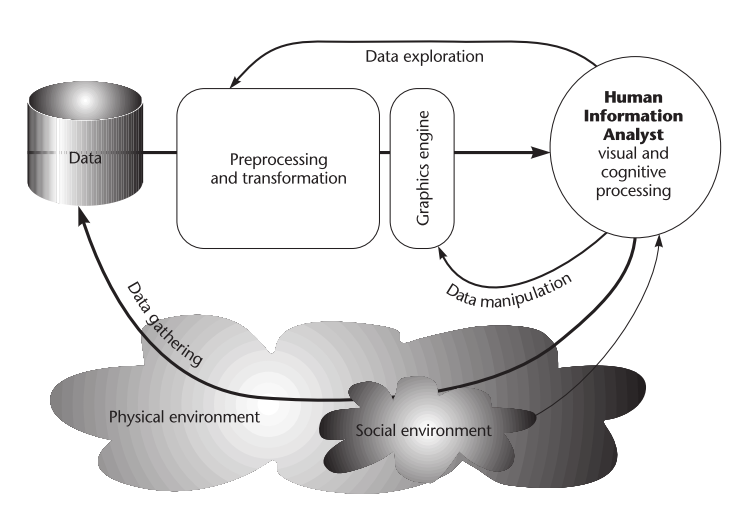
\includegraphics{src/images/VisPipeline}}
    \caption{Visualization Pipeline \cite{Ware2012a}}
    \label{fig:my_label}
\end{figure}


\section{Large Data}

Often, time-oriented datasets are very large and multi-variate which makes it difficult to analyze them. The question is how time-oriented data can be analyzed if the number of data points exceeds the screen resolution. This brings us to the definition of large time-oriented Data. 
We define large time-oriented Data as abstract time-dependent data which is too large to fit on the screen. \cite{Shneiderman2008} Multi-variate time series are time series where one data item holds severable variables at the same point of time \cite{Aigner2011}.
In the following work, we will use time-oriented Data, time-oriented Big Data and Big time-oriented Data equivalently for large time-oriented Data. 

\section{Visualization Tools}